\documentclass[11pt]{article}

% ---- self-contained, clean single-column academic preamble ----
\usepackage[a4paper,top=1in,bottom=1in,left=1.15in,right=1.15in]{geometry}
\usepackage[T1]{fontenc}
\usepackage{lmodern}
\usepackage{microtype}
\usepackage{amsmath,amssymb}
\usepackage{graphicx}
\usepackage{booktabs}
\usepackage[font=small,labelfont=bf,skip=5pt]{caption}
\usepackage{xcolor}
\usepackage[hidelinks]{hyperref}
\usepackage{CJKutf8}
\usepackage{titlesec}
\usepackage{enumitem}

\graphicspath{{figures/}{../results/figures/}}
\setlist{itemsep=2pt,topsep=3pt,parsep=0pt,leftmargin=1.4em}

% generous-but-tidy section spacing
\titlespacing*{\section}{0pt}{2.2ex plus .4ex}{1.0ex}
\titlespacing*{\subsection}{0pt}{1.6ex plus .3ex}{0.6ex}
\titleformat{\section}{\normalfont\large\bfseries}{\thesection.}{0.5em}{}
\titleformat{\subsection}{\normalfont\normalsize\bfseries}{\thesubsection}{0.5em}{}

% paragraph style: indented, no extra skip (classic academic look)
\setlength{\parindent}{1.4em}\setlength{\parskip}{0pt}
\setlength{\emergencystretch}{2em}

% let floats fill pages instead of bunching up
\renewcommand{\topfraction}{0.92}
\renewcommand{\bottomfraction}{0.85}
\renewcommand{\textfraction}{0.08}
\renewcommand{\floatpagefraction}{0.78}
\setcounter{topnumber}{3}\setcounter{totalnumber}{4}

\newcommand{\code}[1]{\texttt{\small #1}}

\title{\vspace{-4ex}\bfseries Reproducing ReLA/GRES on gRefCOCO:\\[2pt]
failure-mode analysis and a post-hoc abstain-or-clarify detector}
\author{Visual Media (Eizo Media-gaku) --- Final Report}
\date{}

\begin{document}
\maketitle
\vspace{-3.5ex}
\begin{center}\small\itshape
Written in English by default; a Japanese version can be produced on request.
\end{center}
\vspace{0.5ex}
\noindent\small Every number and figure in this report is generated by the scripts in
\href{https://github.com/shiinayane/visual-media-gres}{\code{shiinayane/visual-media-gres}}
(\code{scripts/}, \code{results/}) and regenerates from one inference pass per split.
\normalsize

% ------------------------------------------------------------------
\section{Identity}
\begin{tabular}{@{}ll@{}}
\textbf{Name:} WANG Yankai & \textbf{Student ID:} 48256454 \\
\end{tabular}\\[2pt]
\textbf{Department:} \begin{CJK}{UTF8}{min}情報理工学系研究科 電子情報学専攻\end{CJK}\\
\textbf{Laboratory:} \begin{CJK}{UTF8}{min}鈴村研究室\end{CJK} (Suzumura Lab) \quad
\textbf{Research topic:} Vision--Language--Action / human--robot collaboration.

% ------------------------------------------------------------------
\section{Target paper}
\textbf{GRES: Generalized Referring Expression Segmentation} (Liu, Ding, Jiang, \emph{CVPR 2023
Highlight}; network \textbf{ReLA}) generalizes classic Referring Expression Segmentation (RES).
Classic RES assumes \emph{exactly one} target per expression. GRES relaxes this to allow
\textbf{multi-target} expressions (``the two bottles on the left'') and \textbf{no-target}
expressions, whose referent is \emph{absent} from the image. To support and measure this, the
authors release \textbf{gRefCOCO} (COCO train2014 images, RefCOCO-style expressions;
train/val/testA/testB) with an evaluation protocol: \textbf{gIoU} (mean per-sample IoU; a correct
no-target sample scores 1), \textbf{cIoU} (cumulative intersection / cumulative union),
\textbf{N-acc} (no-target recall $=\mathrm{TP}/(\mathrm{TP}{+}\mathrm{FN})$), \textbf{T-acc}
(target retention $=\mathrm{TN}/(\mathrm{TN}{+}\mathrm{FP})$) and \textbf{Pr@\{0.7,0.8,0.9\}}.
ReLA is built on Mask2Former/Detectron2 and reaches state of the art on gRefCOCO.

% ------------------------------------------------------------------
\section{Understanding of the method}
Reading the released code (\code{gres\_model/}), the inference path is:
\begin{enumerate}
\item A \textbf{backbone} (Swin-T/-B or R50) extracts multi-scale visual features and a
\textbf{BERT-base} encoder embeds the expression; the backbone is language-aware (early fusion).
\item An \textbf{MSDeformAttn pixel decoder} builds a high-resolution mask feature map.
\item The \textbf{ReLA decoder} (\code{MultiScaleMaskedReferringDecoder}): 100 learnable
\emph{region queries} iterate through (i)~Region--Image cross-attention, (ii)~a first-layer
Region--Language cross-attention gated by a learned \code{lang\_weight}, and (iii)~region--region
self-attention. Two heads matter at test time: a \emph{minimap/mask} branch yielding a 2-channel
mask \code{pred\_masks}$\in\mathbb{R}^{2\times H\times W}$ (\code{argmax} over channels is the
binary output), and a \emph{no-target (NT) head}---a small MLP applied per region and
\textbf{averaged over all 100 regions} to a single 2-way NT logit.
\item \textbf{Inference} sigmoids both outputs; the evaluator compares \code{argmax} of each to GT.
\end{enumerate}
One observation motivates the rest of the report: the model already exposes two scalars at
inference---the no-target score $\sigma(\mathrm{nt\_logit})$ and the foreground mask
confidence---exactly the quantities needed to decide whether to act, abstain, or ask. ReLA collapses
each with a hard \code{argmax} at $0.5$ and always commits to a mask or ``empty.'' Section~6 keeps the
trained model unchanged and replaces this hard decision with a calibrated abstain-or-clarify policy.

% ------------------------------------------------------------------
\section{Execution environment}
\textbf{Hardware.} NVIDIA \textbf{GB10} (Grace--Blackwell, \textbf{aarch64}), CUDA driver 580 /
\textbf{CUDA 13.0}, compute capability \textbf{sm\_121}, 20 CPU cores, 119\,GB RAM.
The stack the paper targets (torch 1.11 / CUDA 11.8 / detectron2 0.6, Python 3.7--3.9) does not run
on a Blackwell/aarch64 machine, so a modern equivalent was assembled (single GPU, inference only;
Table~\ref{tab:env}).

\begin{table}[t]
\centering\small
\caption{Working software stack for the Blackwell/aarch64 + CUDA-13 server (single GPU, inference).}
\label{tab:env}
\begin{tabular}{@{}l l p{8.3cm}@{}}
\toprule
component & version & note \\
\midrule
Python & 3.11 & venv \\
PyTorch & 2.7.1+cu128 & from the cu128 wheel index (the default PyPI aarch64 wheel is CPU-only) \\
torchvision & 0.22.1 & matched to torch 2.7.1 \\
detectron2 & 0.6 (from source) & CPU-only C++ ops via \code{FORCE\_CUDA=0} (avoids compiling CUDA kernels with the mismatched system nvcc 13.0) \\
numpy & 1.26.4 & pinned \code{<2} for the pycocotools / detectron2 ABI \\
transformers & 4.40.2 & BERT-base text encoder \\
\bottomrule
\end{tabular}
\end{table}

\noindent Two source patches (\code{patches/}, applied by \code{setup.sh}), both forced by the
Blackwell + CUDA-13 mismatch:
\begin{enumerate}
\item \textbf{MSDeformAttn fallback.} The hand-written CUDA op cannot be compiled (system nvcc 13.0
vs torch cu128/12.8); I fall back to ReLA's own pure-PyTorch \code{ms\_deform\_attn\_core\_pytorch}
(\code{F.grid\_sample}), the reference implementation---numerically close, not bit-identical.
\item \textbf{sm\_121 nvrtc fix.} \code{spatial\_shapes.prod(1)} on int64 falls to the nvrtc
jiterator, whose cu128 build rejects \code{-arch=compute\_121}; I replace it with the identical
elementwise product \code{shapes[:,0]*shapes[:,1]} (precompiled kernel).
\end{enumerate}

\noindent\textbf{Baseline reproduction (gRefCOCO val, Swin-T, 14{,}229 expressions):}
gIoU\,=\,55.76, cIoU\,=\,55.64, N-acc\,=\,46.3\%, T-acc\,=\,99.9\%, Pr@0.7\,=\,66.5. The paper reports
Swin-T cIoU 57.73 / gIoU 56.86, so the result lands within $\sim$1--2 points---a faithful
reproduction; the small gap is consistent with the \code{grid\_sample} fallback and single-GPU
evaluation and does not affect any conclusion below. Inference runs at $\approx$0.24\,s/sample; one
pass dumps compact per-sample signals to \code{results/*.pkl} and all downstream analysis is offline.

% ------------------------------------------------------------------
\section{Failure case analysis}
I study two failure conditions on gRefCOCO's official splits, so each claim is a measured rate, not
an anecdote. F1 (no-target) is analysed on \textbf{val} (63\% of its samples are no-target---the
ideal stress test); F2 (multi-target) on \textbf{testA}, the split that contains a single-target
baseline to compare against.

\subsection{F1 --- No-target hallucination (primary)}
\textbf{Setup.} Restrict to the no-target subset of val ($\mathrm{gt\_nt}{=}$True, $n{=}8{,}905$, 63\%
of val). A \emph{hallucination} is a no-target sample on which the model still emits a non-empty mask.

\smallskip\noindent\textbf{Result.} The model hallucinates on \textbf{53.7\%} of no-target samples
(4{,}784/8{,}905); N-acc\,=\,46.3\%. The opposite error is almost absent: T-acc\,=\,99.9\% (only 7 of
5{,}324 present-target samples are wrongly called empty). The hallucinated masks are not small
artefacts---median 7.2\% of the image (mean 9.1\%), mean foreground confidence 0.68: the model tends
to be \emph{wrong with high confidence}.

\smallskip\noindent\textbf{Mechanism.} Figure~\ref{fig:f1a} plots the model's own no-target score
$s_\mathrm{nt}=\sigma(\mathrm{nt\_logit})_1$ for present vs absent referents. Present-target samples
pile up at $s_\mathrm{nt}\!\approx\!0$ (mean 0.012). Absent-referent samples are \textbf{bimodal}: a
high mode ($\sim$37\% above 0.9, correctly ``no target'') and a \textbf{low mode} ($\sim$38\%
collapsing to $s_\mathrm{nt}\!\approx\!0$, inside the present distribution), so overall 53\% fall below
the $0.5$ threshold (the empty-subset mean 0.48 is the average of two modes, not a typical value).
Architecturally the NT head is a \emph{single} scalar \textbf{averaged over all 100 region queries};
a plausible account is that a few regions confidently matching a salient distractor pull the mean
below $0.5$ and a mask is committed. I logged only the pooled $s_\mathrm{nt}$, not per-region logits,
so this is consistent with the architecture but not directly verified (Section~8). For a system that
acts on language, this high-confidence false positive is the most costly error.

\begin{figure}[t]
\centering
\begin{minipage}[t]{0.49\linewidth}\centering
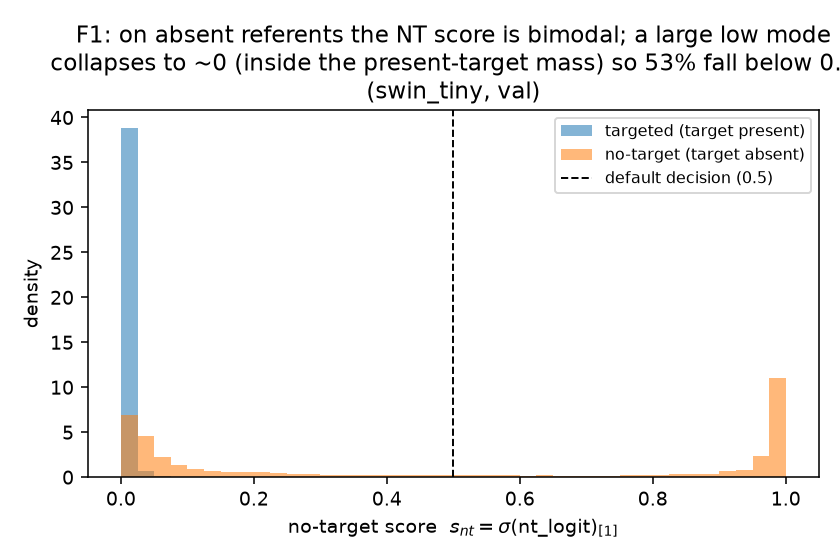
\includegraphics[width=\linewidth]{F1_nt_score_hist.png}
\caption{No-target score for present vs absent referents. On absent referents the score is bimodal;
the large low mode collapses inside the present-target distribution, so 53\% fall below $0.5$ and a
mask is committed.}
\label{fig:f1a}
\end{minipage}\hfill
\begin{minipage}[t]{0.49\linewidth}\centering
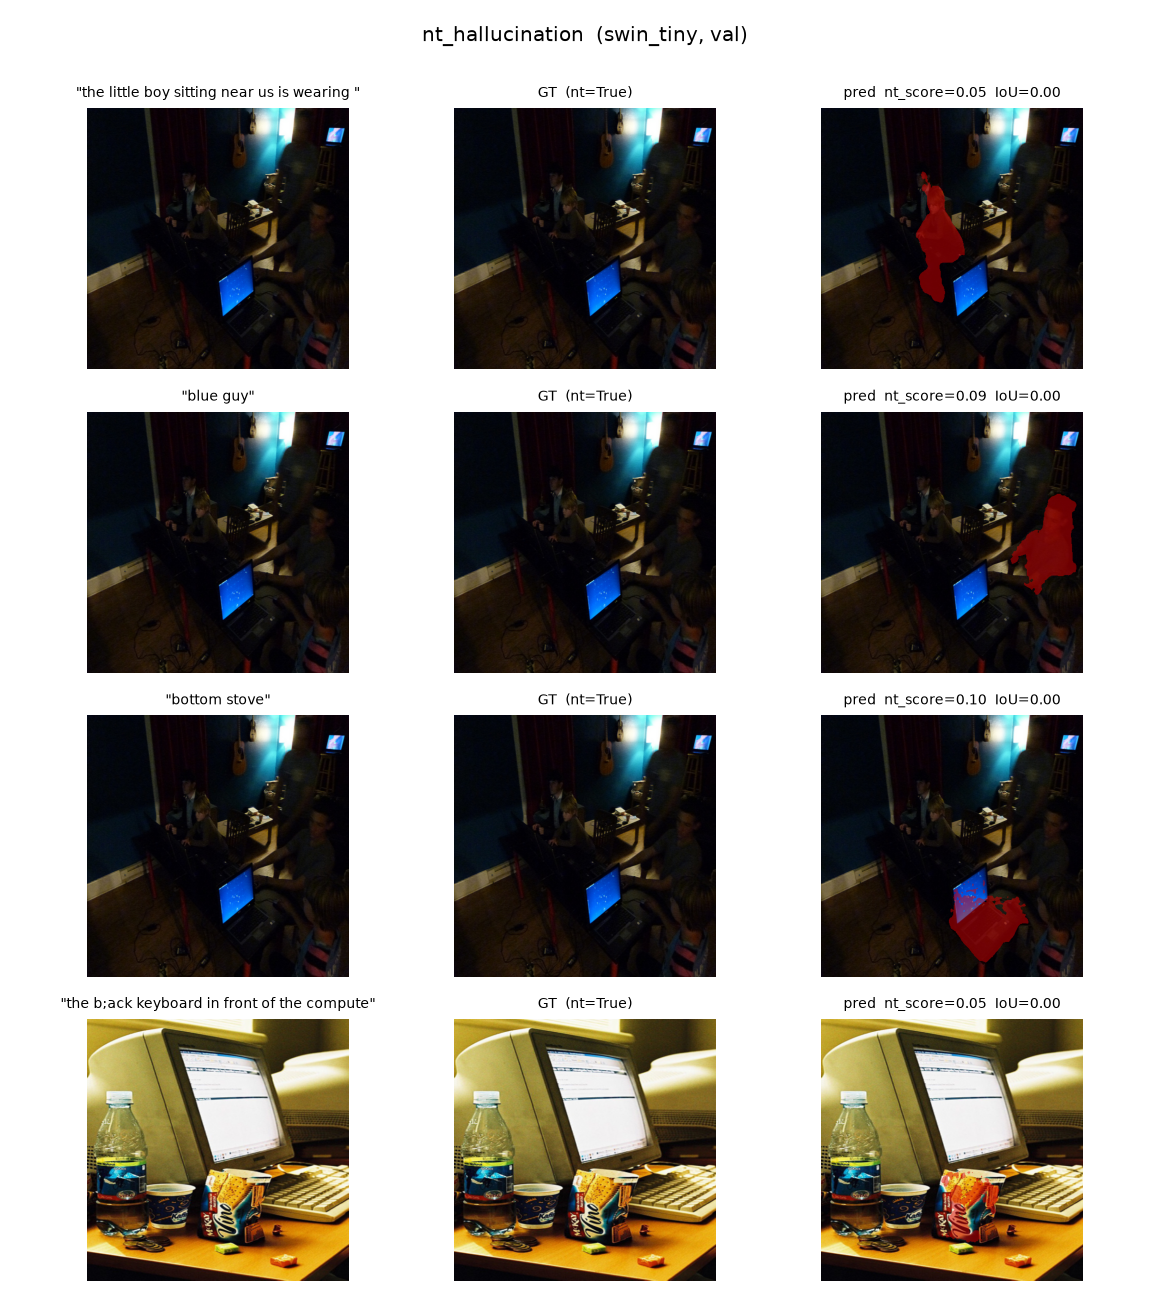
\includegraphics[width=\linewidth]{qual_nt_hallucination_swin_tiny.png}
\caption{Each row: one \emph{no-target} expression (left), the empty ground truth (middle), and the
model's confident hallucinated mask in red (right).}
\label{fig:f1b}
\end{minipage}
\end{figure}

\subsection{F2 --- Multi-target under-segmentation}
\textbf{Setup.} I use \textbf{testA} because (unlike val, whose targeted expressions are all
multi-instance) it has a single-instance baseline (5{,}917 one-target, 5{,}940 two-target, 2{,}895
three-or-more). For each GT instance I record coverage $=|\mathrm{pred}\cap\mathrm{inst}|/|\mathrm{inst}|$,
call it a \emph{hit} if $\geq0.5$, and report per-instance recall.

\smallskip\noindent\textbf{Result (two effects).} (i)~Per-instance recall is \textbf{flat from one to
two targets}---0.868 (single) vs 0.881 (two)---then \textbf{collapses to 0.594 at $\geq$3 targets}.
(ii)~Independently of count, coverage within a multi-target expression is \textbf{very uneven}: the
best-covered instance averages 0.92 but the worst only 0.58, and the model \textbf{drops at least one
instance entirely in 37.8\%} of multi-target testA samples (26.1\% on val). The under-segmentation is
thus not ``two worse than one on average''; it is a \textbf{capacity ceiling at $\geq$3 targets} plus
\textbf{lopsided coverage} sacrificing the less salient instance.

\smallskip\noindent\textbf{Mechanism.} ReLA predicts a single 2-channel ``target'' mask via an
\code{einsum} over per-region minimap weights. One mask can represent one region, or two when the soft
weighting is shared, but cannot spread mass across many disjoint instances---matching both the sharp
drop at $\geq$3 and the dropped weaker instance within a pair.

\begin{figure}[t]
\centering
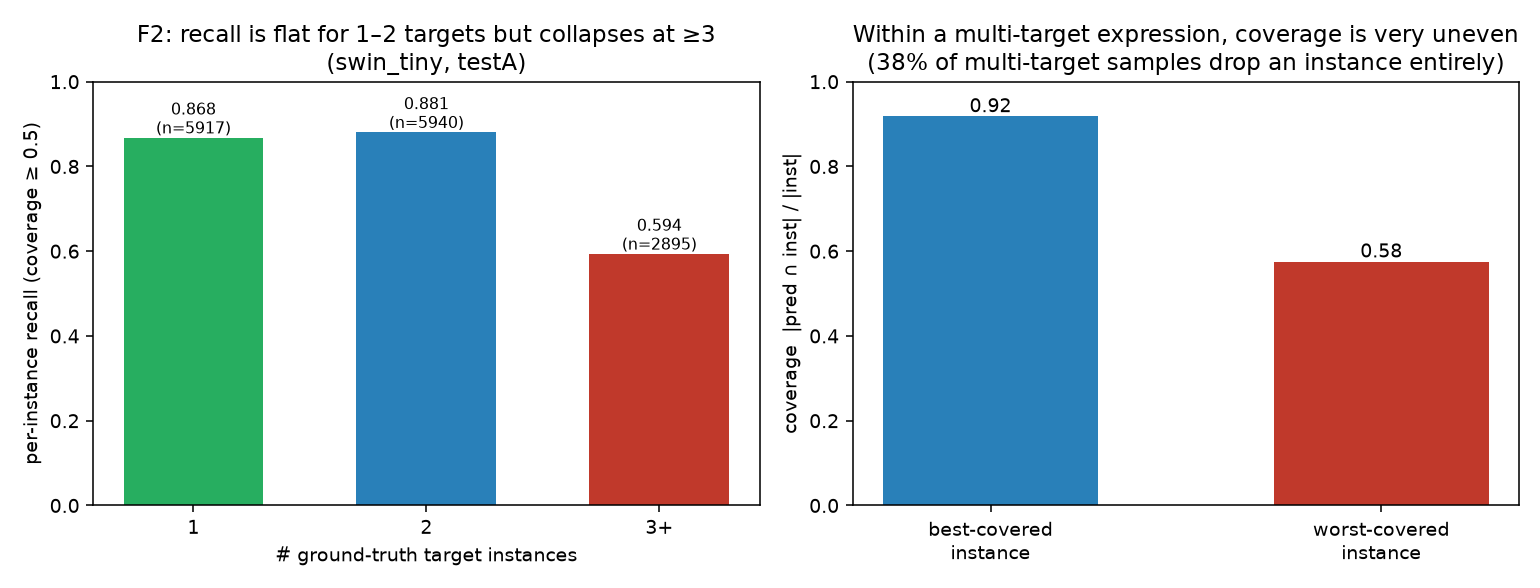
\includegraphics[width=0.86\linewidth]{F2_recall_by_count.png}
\caption{testA. \emph{Left:} per-instance recall is flat for 1--2 targets (0.87, 0.88) but collapses
at $\geq$3 (0.59). \emph{Right:} within a multi-target expression the best instance is covered at 0.92
but the worst at only 0.58 (38\% of samples drop one entirely).}
\label{fig:f2a}
\end{figure}

\begin{figure}[t]
\centering
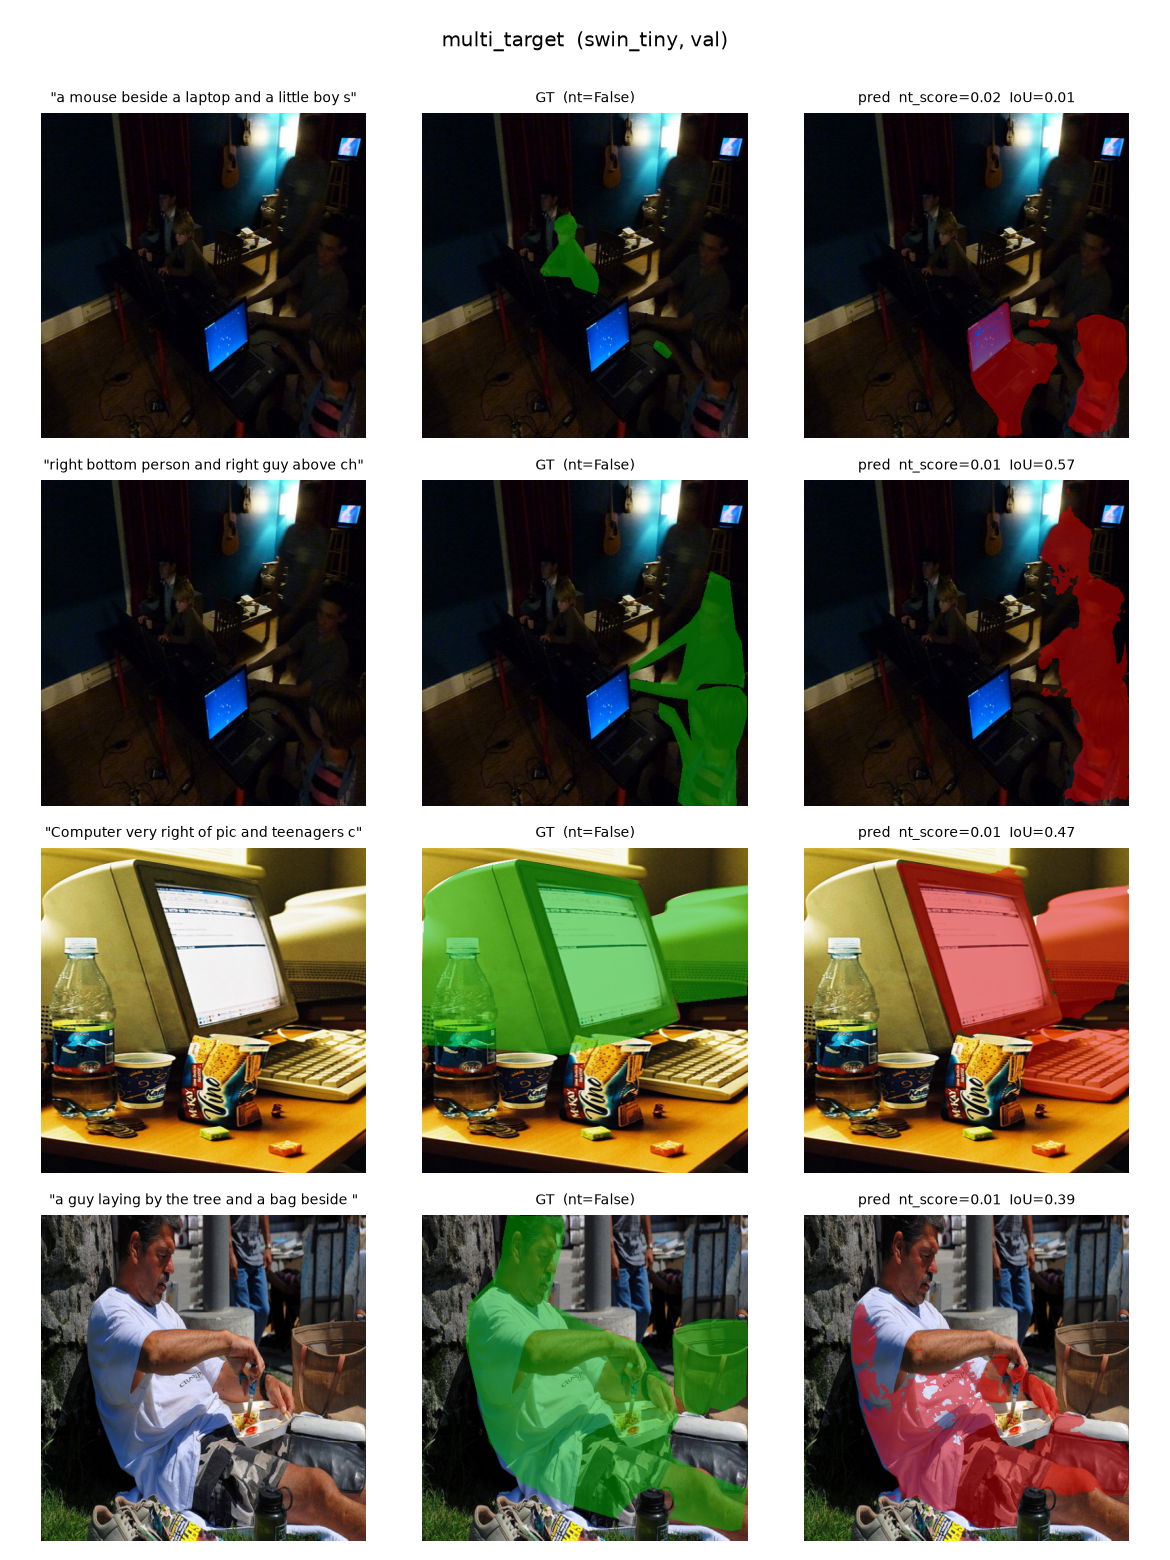
\includegraphics[width=0.62\linewidth]{qual_multi_target_swin_tiny.png}
\caption{Qualitative multi-target cases. Each row is one expression; ground-truth instances in green
(middle), prediction in red (right). The model frequently captures the salient instance and drops the
other.}
\label{fig:f2b}
\end{figure}

% ------------------------------------------------------------------
\section{Improvement: a post-hoc abstain-or-clarify detector}
Motivated by my research on human--robot collaboration---where a system facing an unsatisfiable or
ambiguous instruction should ask or abstain rather than commit---I keep the trained model unchanged
(no retraining) and replace its hard \code{argmax} with a calibrated policy. For each sample I define
$s_\mathrm{abstain} = \max(s_\mathrm{nt},\, 1-\overline{\mathrm{mask\_conf}})$, high when the model
leans ``no target'' \emph{or} its committed mask is low-confidence. The policy is:
\begin{itemize}
\item $s_\mathrm{abstain}\!\geq\!\tau \Rightarrow$ \textbf{ABSTAIN} (emit empty; scored as no-target);
\item else if a mask has $\geq$2 connected components, the largest covering $<\rho$ of the area
$\Rightarrow$ \textbf{CLARIFY} (``did you mean A or B?'');
\item else $\Rightarrow$ \textbf{COMMIT} the mask.
\end{itemize}
$\tau$ is calibrated on val (max gIoU) and applied unchanged to held-out testA. I also report a safety
point $\tau_\mathrm{safe}$: the most aggressive abstention keeping T-acc\,$\geq$\,0.95. CLARIFY has no
benchmark counterpart, so for scoring I keep the best-guess mask and report its trigger count
separately. Calibration gives $\tau=0.23$ (gIoU-optimal), $\tau_\mathrm{safe}=0.38$, $\rho=0.7$.

% ------------------------------------------------------------------
\section{Before/after comparison}
$\tau$ is calibrated on \textbf{val} and applied \textbf{unchanged} to held-out \textbf{testA}
(Tables~\ref{tab:val}--\ref{tab:testa}; trade-off in Fig.~\ref{fig:tradeoff}).

\begin{table}[t]
\centering\small
\begin{minipage}[t]{0.49\linewidth}\centering
\caption{gRefCOCO \textbf{val} ($n{=}14{,}229$). \emph{In-sample}: $\tau$ is both chosen and scored
here, so read this as the calibration curve, not a result.}
\label{tab:val}
\begin{tabular}{@{}lcccc@{}}
\toprule
op.\ point & gIoU & cIoU & N-acc & T-acc \\
\midrule
baseline & 55.76 & 55.64 & 46.3 & 99.9 \\
safe $0.38$ & \textbf{66.9} & \textbf{58.2} & \textbf{65.0} & 95.1 \\
gIoU-opt $0.23$ & 74.1 & 52.4 & 87.7 & 62.5 \\
\bottomrule
\end{tabular}
\end{minipage}\hfill
\begin{minipage}[t]{0.49\linewidth}\centering
\caption{gRefCOCO \textbf{testA} (held out, $\tau$ transferred unchanged; $n{=}19{,}200$). The honest
evaluation.}
\label{tab:testa}
\begin{tabular}{@{}lcccc@{}}
\toprule
op.\ point & gIoU & cIoU & N-acc & T-acc \\
\midrule
baseline & 65.03 & 65.42 & 50.6 & 99.0 \\
safe $0.38$ & \textbf{65.9} & 64.5 & \textbf{63.3} & 90.6 \\
gIoU-opt $0.23$ & 54.1 & 49.3 & 83.6 & 54.6 \\
\bottomrule
\end{tabular}
\end{minipage}
\end{table}

On testA, with $\tau$ transferred unchanged, the detector is best described as a \textbf{safety
re-weighting} rather than a segmentation-quality gain: the safe point raises N-acc by 12.7 points
(50.6$\to$63.3) at a cost of 8.4 points of T-acc (99.0$\to$90.6), with overlap metrics essentially
unchanged (gIoU $+0.9$, within the reproduction gap; cIoU $-1.0$). What it buys is a tunable,
calibrated willingness to abstain on unsatisfiable instructions at a bounded retention cost. The
aggressive gIoU-optimal $\tau$ \emph{does not transfer}: tuned to val's 63\%-no-target prior, on the
23\%-no-target testA it over-abstains and lowers gIoU by 11 points. Hence only the T-acc-constrained
point transfers safely, and a practical detector would calibrate $\tau$ to the deployment base-rate.
The \textbf{CLARIFY} branch (separate from abstention) fired on 1{,}131 val / 1{,}712 testA committed
predictions at $\tau{=}0.23$---multi-component masks for which ``which one?'' is a reasonable
alternative; an illustrative remedy for F2, reported as a trigger count since gRefCOCO has no
clarification label.

\begin{figure}[t]
\centering
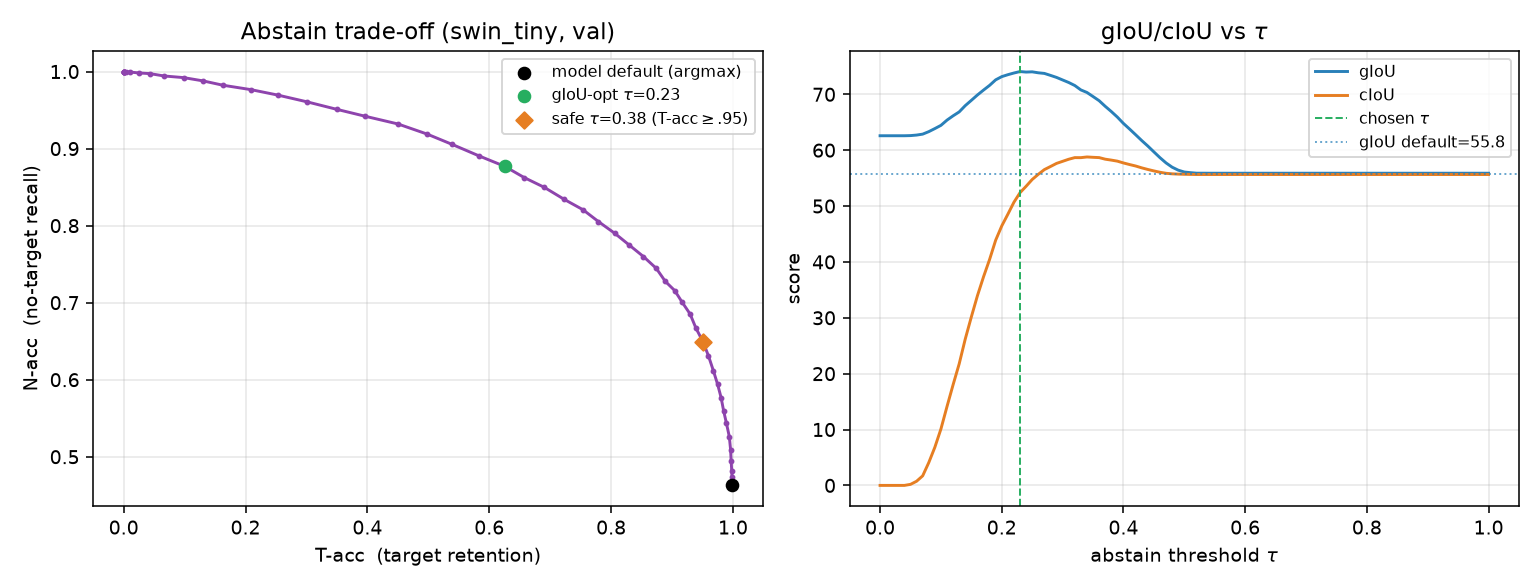
\includegraphics[width=0.86\linewidth]{abstain_tradeoff.png}
\caption{Abstain/clarify trade-off, calibrated on val. \emph{Left:} N-acc vs T-acc as $\tau$ sweeps;
the default \code{argmax} point (black) sits at the extreme no-abstention corner, the safe (orange)
and gIoU-optimal (green) points move up the frontier. \emph{Right:} gIoU and cIoU vs $\tau$, both
peaking above the default (dotted).}
\label{fig:tradeoff}
\end{figure}

% ------------------------------------------------------------------
\section{Limitations}
\begin{itemize}
\item Inference-only on the frozen Swin-T checkpoint (Swin-B downloaded but, per the resource
guideline, not evaluated); with no retraining the detector reuses signals, not fixes the F2 bias.
\item The \code{grid\_sample} MSDeformAttn fallback is the reference op (close, not identical); the
$\sim$1-point baseline gap is plausibly but not provably benign.
\item The F1 mechanism is a hypothesis: I logged only the pooled $s_\mathrm{nt}$, not per-region NT
logits, so the averaging-dilution account is consistent with, but not proof of, the architecture.
\item $\max(s_\mathrm{nt},1-\mathrm{mask\_conf})$ is a simple interpretable rule with correlated
terms; a learned calibrator over $\{s_\mathrm{nt},\mathrm{mask\_conf},\mathrm{area},\#\mathrm{comp}\}$
would likely do better.
\item On held-out data the detector is a safety re-weighting, not a quality gain, and a single global
$\tau$ depends on the no-target base-rate. The CLARIFY trigger is a geometric heuristic reported only
as a count (no clarification label; it does not yet read the expression).
\end{itemize}

% ------------------------------------------------------------------
\section{Generative-AI usage}
I used a generative-AI coding assistant (Anthropic's Claude, via the Claude Code CLI) throughout, and
disclose it as follows. \textbf{The AI assisted with:} debugging the Blackwell/CUDA-13 environment and
proposing the working stack and the two source patches (Section~4); writing the bulk of the analysis
code in \code{scripts/} (inference loop, metric port, failure-mode and detector scripts, plotting);
running the experiments; and drafting report text from the resulting numbers. \textbf{I am responsible
for:} selecting the paper and the direction (the abstain-or-clarify framing tied to my HRC research);
reviewing the code and setup; checking every reported number and figure against the generated tables;
requesting the corrections from an internal review (e.g.\ re-centring F2 on testA; reporting held-out
rather than in-sample detector results); and editing the report into final form. A detailed running
log is in \code{GENAI\_USAGE\_LOG.md}.

% ------------------------------------------------------------------
\section{Discussion}
The two failure modes share an origin: ReLA makes a single hard decision at inference (one mask, one
$0.5$ no-target threshold), whereas the generalized task is partly about \emph{uncertainty}---whether
a referent exists at all, and how many. The no-target and multi-target subsets are exactly where
committing to a single \code{argmax} is the wrong default. The detector adds no capacity; it reuses
the uncertainty the model already encodes and turns it into three actions (act, abstain, ask), giving
a calibrated, tunable abstention at a bounded retention cost that transfers to a held-out split. For a
benchmark aimed at human--robot use, this argues for an explicit abstain/clarify option in how
grounding models are both \emph{scored} and \emph{operated}, since these are the cases where a
confident-but-wrong mask is most costly. The gains are modest and prior-dependent; natural next steps
are a small learned calibrator over the four signals, an expression-aware CLARIFY trigger, and an
abstention-aware metric (e.g.\ risk--coverage) reported alongside gIoU/cIoU.

\vspace{1.5ex}
\noindent\rule{\linewidth}{0.3pt}\\[0.4ex]
{\small\emph{Citation:} Chang Liu, Henghui Ding, Xudong Jiang. ``GRES: Generalized Referring
Expression Segmentation.'' \textbf{CVPR 2023} (Highlight). arXiv:2306.00968.}

\end{document}
